\section{Графическое изображение матожидания критерия}
Вычислим матожидание от имеющегося векторного критерия \eqref{eq:player_criterion}
, где $x$ и $y$ возьмём как случайные величины с распределениями \eqref{eq:probability_1}
и соответсвующими обозначениями велечин $p$ и $q$. В таком случае имеем:

\begin{gather*}
	\mathbb{E}_x [F(x,y)]=
	\Big(
		\dfrac{yq}{2};
		\dfrac{1-q}{y}
	\Big)
	\\
	\mathbb{E}_{xy} [F(x,y)]=
	\big(
		\dfrac{q(1+p)}{2};
		\dfrac{(1-q)(2-p)}{2}
	\Big)
\end{gather*}

Рассмотрим это как множество точек на плоскости $X,Y$ зависящие от двух параметров $(p,q)\in[0,1]^2$

$$
	\begin{cases}
		x = \dfrac{q(1 + p)}{2} \\
		y = \dfrac{(1 - q)(2 - p)}{2}  
	\end{cases}
	\Rightarrow
	\begin{cases}
		q = \dfrac{2x}{1 + p} \\
		y = \dfrac{(1 - \dfrac{2x}{1 + p})(2 - p)}{2}		
	\end{cases}
	\Rightarrow
	\begin{cases}
		q = \dfrac{2x}{1 + p} \\
		y = \dfrac{(1 + p - 2x)(2 - p)}{2(1 + p)}
	\end{cases}
$$

Найдём максимальные значения, которые может принимать $y(x, p)$ при фиксированном $x$:

$$
	\dfrac{\partial y(x, p)}{\partial p}=\frac{3x}{(p+1)^2} - \frac{1}{2} = 0 
	\Rightarrow
	p = \sqrt{6x} - 1
$$

Введём обозначение $p_0 = \sqrt{6x} - 1$. Поскольку область определения 
$p_0 \in [0, 1]$, то $p_0 = 1 \Rightarrow x = \frac{2}{3}$ и 
$p_0 = 0 \Rightarrow x = \frac{1}{6}$
 
$$
	y_{max}(x) = 
	\begin{cases}
		\max \{ y(x, 0), \: y(x, 1), \: y(x, p_0) \}, & 
		x \in \big[ \frac{1}{6}, \frac{2}{3} \big]
		\\
		\max \{ y(x, 0), \: y(x, 1) \}, &
		x \in \big[0, \frac{1}{6} \big] \cap \big[\frac{2}{3}, 1\big]
	\end{cases}
$$

учитывая, что
$
	y(x, 0) = 1 - 2x, \;
	y(x, 1) = \dfrac{1 - x}{2}, \;  	
	y(x, p_0) = \dfrac{(\sqrt{6x} - 2x)(3 - \sqrt{6x})}{2 \sqrt{6x}}
$
получим уравнения верхней и нижней огибающей области на графике ниже.

\begin{gather*}
	y_{min}(x) =
	\begin{cases}
		\dfrac{1 - x}{2}, & x \in \big[0, \frac{1}{3} \big] 
		\\
		1 - 2x, & x \in \big( \frac{1}{3}, 1\big]
	\end{cases}
	\\
	y_{max}(x) =
	\begin{cases}
		1 - 2x, & x \in \big[0, \frac{1}{6} \big] 
		\\
		\dfrac{(\sqrt{6x} - 2x)(3 - \sqrt{6x})}{2 \sqrt{6x}}, &
		x \in \big(\frac{1}{6}, \frac{2}{3} \big]
		\\
		\dfrac{1 - x}{2}, & x \in \big(\frac{2}{3}, 1 \big]
	\end{cases}
\end{gather*}


В предыдущем пункте мы установили \eqref{State:opt_strat_1} что любая пара
$(p^{*}, q^{*}) \in [0, 1]^{2}$ является оптимальной. Теперь для всех
оптимальных стратегий т.е. пар $(p^{*}, q^{*}) \in [0, 1]^{2}$ изобразим на графике
значения матожидания векторного критерия в этой точке.

\begin{figure}[H]
	\centering
	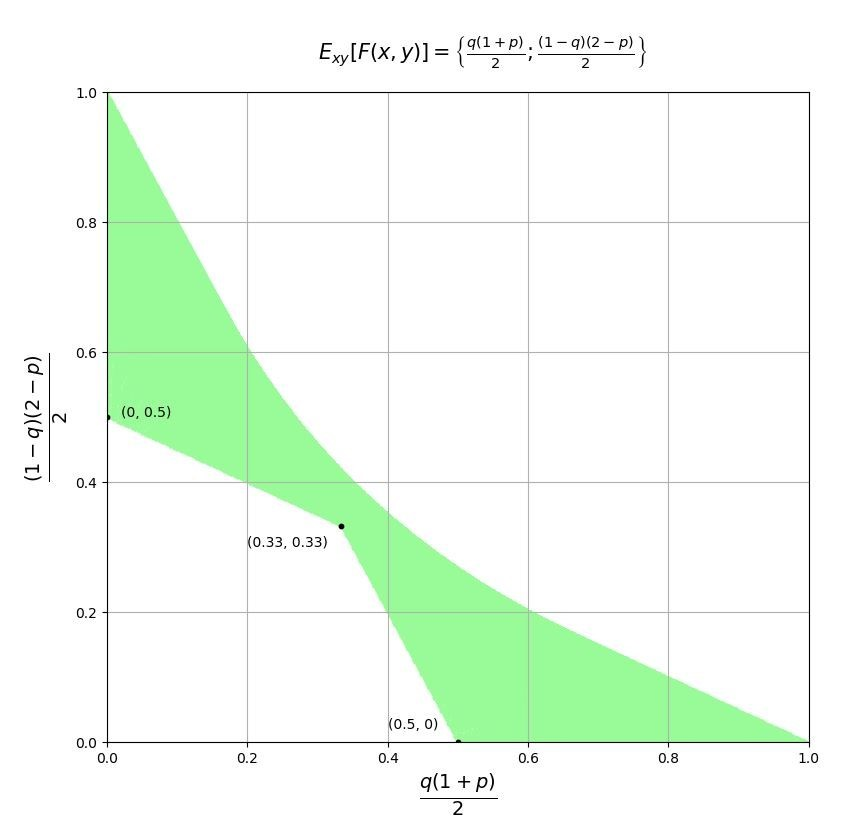
\includegraphics[scale=0.8]{part_2/graf_1_2}
	\caption{Матожидание векторного критерия}
\end{figure}